\documentclass[border=10pt]{standalone}

\usepackage{tikz}
\usepackage{tikzsymbols}
\usetikzlibrary{calc,patterns,shapes.geometric}

\def\centerarc[#1](#2)(#3:#4:#5){\draw[#1] ($(#2)+({#5*cos(#3)},{#5*sin(#3)})$) arc (#3:#4:#5);}

\begin{document}
	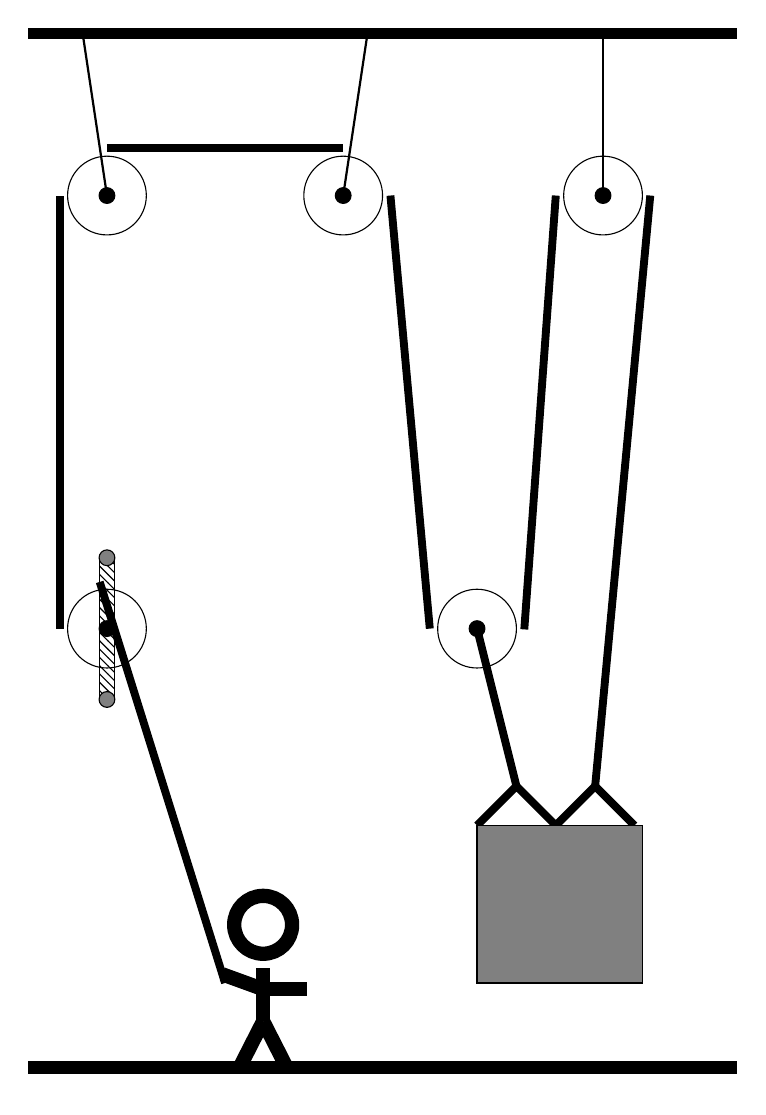
\begin{tikzpicture}
		%%%%% START %%%%%
		\draw[fill=black] (-3, 10) rectangle (6, 10.125);
		
		\draw (1, 8.0) circle (0.5);
		\draw[fill=black] (1, 8.0) circle (0.1);
		\draw[thick] (1, 8.0) -- (1.3, 10);
		
		\draw (4.3, 8.0) circle (0.5);
		\draw[fill=black] (4.3, 8.0) circle (0.1);
		\draw[thick] (4.3, 8.0) -- (4.3, 10);
		
		\draw (2.7, 2.5) circle (0.5);
		\draw[fill=black] (2.7, 2.5) circle (0.1);
		
		\draw[line width=1mm]  (2.7, 0) -- (3.2, 0.5) -- (3.7, 0) -- (4.2, 0.5) -- (4.7, 0);
		\draw[fill=black!50] (2.7, 0) rectangle (4.8, -2);
		
		\draw (-2, 8.0) circle (0.5);
		\draw[fill=black] (-2, 8.0) circle (0.1);
		\draw[thick] (-2, 8.0) -- (-2.3, 10);
		
		\draw (-2, 2.5) circle (0.5);
		\draw[fill=black] (-2, 2.5) circle (0.1);
		\draw[pattern=north west lines, pattern color=black] (-2.1, 3.4) rectangle (-1.9, 1.6);
		\draw[fill=black!50] (-2, 3.4) circle (0.1);
		\draw[fill=black!50] (-2, 1.6) circle (0.1);
		
		\draw[line width=1mm](-0.5, -2) -- (-2.092, 3.093);
		\centerarc[line width=1mm](-2, 2.5)(180:210:0.6);
		\draw[line width=1mm](-2.6, 2.5) -- (-2.6, 8.0);
		\centerarc[line width=1mm](-2, 8.0)(90:180:0.6);
		
		\draw[line width=1mm](-2, 8.6) -- (1, 8.6);
		\centerarc[line width=1mm](1, 8.0)(0:90:0.6);
		\draw[line width=1mm](1.6, 8.0) -- (2.1, 2.5);
		\centerarc[line width=1mm](2.7, 2.5)(180:370:0.6);
		\draw[line width=1mm] (3.3, 2.49) -- (3.7, 8.0);
		\centerarc[line width=1mm](4.3, 8.0)(0:180:0.6);
		\draw[line width=1mm](4.2, 0.5) -- (4.9, 8.0);
		\draw[line width=1mm] (3.2, 0.5) -- (2.7, 2.5);
		
		\node at (0, -2) {\Strichmaxerl[10][-20][0]};
		
		\draw[fill=black] (-3, -3) rectangle (6, -3.15);
		%%%%% END %%%%%
	\end{tikzpicture}
\end{document}